\chapter{$H^+\to tb$ analysis overview}
\label{chapter:Htbanalysis}

The discovered scalar particle in 2012 raises whether it is the Higgs boson of the~\acrshort{SMlabel} or part of an extended scalar sector. Charged Higgs bosons\footnote{In the following, charged Higgs bosons are denoted $H^+$, with the charge-conjugate $H^-$ always implied. Similarly, the difference between quarks and antiquarks $q$ and $\bar{q}$ is generally understood from the context, so that $H^+\to tb$ means both $H^+\to t\bar{b}$ and $H^-\to \bar{t}b$.} are predicted in several extensions of the~\acrshort{SMlabel} that add a second doublet or triplets to the scalar sector, as discussed in Section~\ref{section:BSM}.\\

The~\acrshort{ATLASlabel} and CMS collaborations have searched for charged Higgs bosons in $pp$ collisions at $\sqrt{s}$= 7, 8 and 13~TeV with data samples ranging from 2.9 to 36 fb$^{-1}$, probing the mass range below the top-quark mass in the $\tau\nu$~\cite{Hplustaunu12,Hplustaunu13,Hplustaunu15,Hplustaunu12CMS,Hplustaunu15CMS,Hplustaunu18}, $cs$~\cite{Hpluscs2013,Hpluscs2015}, $cb$~\cite{HpluscbCMS,Hpluscb2022},$WA$ ($A$ pseudo-scalar) decay modes, as well as above the top-quark mass in the $\tau\nu$ and $tb$ decay modes~\cite{Hplustaunu12,Hplustaunu13,Hplustaunu15,Hplustaunu12CMS,Hplustaunu18,Hplustb2015,Sirunyan_2020,Hplustb21CMS,ATLASHptb2018}. In addition, $H^+\to WZ$ decays were searched for in the vector-boson-fusion production mode~\cite{HplusWZ15,HplusWZ15CMS}. \acrshort{ATLASlabel} has also set limits on the $H^+$ production in a search for di-jet resonances in events with an isolated lepton using the Run~2 dataset~\cite{Hplusdijet20}. No evidence of charged Higgs bosons was found in any of these searches.\\
    
The analysis presented in this thesis is performed with the full Run~2 proton-proton collision data of 139 fb$^{-1}$ at $\sqrt{s}$=13~TeV. The results of this search are public~\cite{Hpluspaper}, and were later interpreted to be used in an~\acrshort{ATLASlabel} effort to combine dark matter results~\cite{Hpluscomb}:

\begin{itemize}
    \item ATLAS Collaboration, \textit{Search for charged Higgs bosons decaying into a top quark and a bottom quark at $\sqrt{s}$=13~TeV with the ATLAS detector}, JHEP 06 (2021) 145
    
    \item ATLAS Collaboration, \textit{Combination and summary of ATLAS dark matter searches using 139 fb$^{-1}$ of $\sqrt{s}$=13~TeV $pp$ collision data and interpreted in a two-Higgs-doublet model with a pseudoscalar mediator}, ATLAS-CONF-2021-036
\end{itemize}

This chapter describes the $H^+\to tb$ analysis motivation, challenges and strategy. After a short introduction, the event selection is presented followed by the description of the modelling of the signal and background processes. Then, the analysis strategy and a summary of the systematic uncertainties are given.

\section{Introduction}
The analysis searches for charged Higgs bosons heavier than the top quark and decaying into a top and bottom quark. At the~\acrshort{LHClabel}, charged Higgs bosons in this mass range are expected to be produced primarily in association with a top quark and a bottom quark~\cite{CYRM-2017-002}, illustrated in Figure~\ref{Hplustb:feynman1}.\\

\begin{figure}[htbp]
    \RawFloats
    \begin{center}
    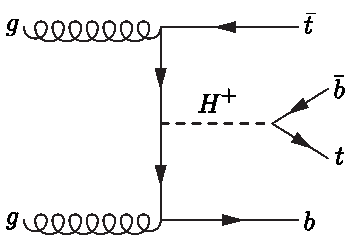
\includegraphics[width=0.5\textwidth]{HPLUSTB/feynmansmall.pdf}
    \caption{
        Leading-order Feynman diagram for the production of a heavy charged Higgs boson in association with a top antiquark and a bottom quark, as well as its decay into a top quark and a bottom antiquark.
    }
    \label{Hplustb:feynman1}
    \end{center}
\end{figure}

The signal consists in two top quarks and two bottom quarks, once of each produced in association with the $H^+$ and the other from its decay. For convenience, the typical classification for \ttbar\ events is used, based in the decay of the involved top quarks. The main decay mode for top quarks is to a $W$ and a $b$-quark, with the former decaying either leptonically (to leptons) or hydronically (to a pair of quarks). This yields to four possible diagrams depending on the decay of each top but three different types of final states with different decay rates~\cite{pdg}: the all-hadronic final state where both $W$-bosons decay hadronically (45.7\%), the dileptonic mode where both $W$-bosons decay leptonically\footnote{Hadronically decaying $\tau$ leptons are included in the numbers.} (10.5\%) and the lepton+jets (semi-leptonic) final state, in which one $W$-boson decays hadronically and one leptonically (43.8\%).\\

In the scope of the analysis, the lepton+jets channel is studied as offers large statistics with a relatively clean topology, as the lepton in the final state allows to suppress the multi-jet background. In addition, the full event can be kinematically reconstructed, since only one neutrino is present and can be determined with \MET. The dilepton channel was studied in the past~\acrshort{ATLASlabel} searches, with low impact in the final result. Aside, the lepton+jets channel could be further split into a resolved (low \pT) regime and a boosted regime, in order to optimise high \pT\ regimes that lead to collimated partons that cannot be resolved with the standard jet collections. The final state is depicted in Figure~\ref{Hplustb:feynman2}\\

\begin{figure}[htbp]
    \RawFloats
    \begin{center}
    \subfloat[]{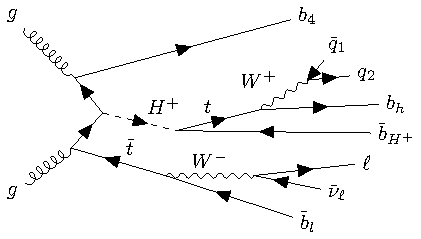
\includegraphics[width=0.47\textwidth]{HPLUSTB/feynman_had.pdf}} \quad
    \subfloat[]{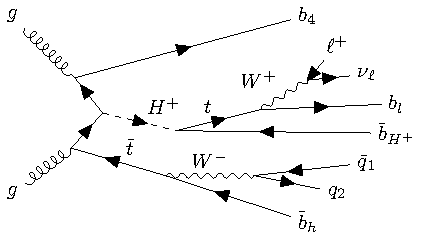
\includegraphics[width=0.47\textwidth]{HPLUSTB/feynman_lep.pdf}}
    \caption{
        Leading-order Feynman diagrams for the production and decay of a heavy charged Higgs boson into a top and a bottom quark, with the former decaying hadronically (a) or leptonically (b), in the signal-lepton final state.
    }
    \label{Hplustb:feynman2}
    \end{center}
\end{figure}

The detector signature is chosen to include exactly one isolated lepton $\ell$, considering only electrons and muons. Nonetheless, the $\tau$ leptons decaying into electrons or muons are included. As six quarks are present in the final state, six jets are expected to be present in the final state with at least four of them originating from a $b$-quark. Although the recommendations available at the time were based on EMTopo jets, the performance improvements with PFlow jets would have benefited the analysis, as the $b$-tagging is one important part of the selection.\\

The targeted final state complexity originates from the dominant \ttbar\ production with additional jets (\ttjets). In particular, \ttb\ is the main irreducible background for which an example diagram is shown in Figure~\ref{Hplustb:feynman3}. Hence, the correct modelling of this process is key for the analysis and unfortunately, it is poorly constrained by data measurements and has large theory uncertainties.\\


\begin{figure}[htbp]
    \RawFloats
    \begin{center}
    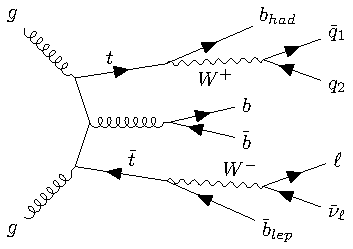
\includegraphics[width=0.5\textwidth]{HPLUSTB/feynman_ttbar.pdf}
    \caption{
        Leading-order Feynman diagram for the \ttbar\ production with a radiated $b\bar{b}$ in the single-lepton final state.
    }
    \label{Hplustb:feynman3}
    \end{center}
\end{figure}

As a summary of the analysis strategy, the first step is the event selection, where a first phase space is chosen to enhance the $H^+$ signal contribution but also includes events to study the~\acrshort{SMlabel} background. Events are then split into signal-enriched categories (signal region, SR) and signal-depleted categories (control region, CR). The control regions are used to extract data-driven corrections for the \ttbar\ modelling while for the signal regions, a NN is used to separate signal and background. The signal regions are used in a combined profile-likelihood fit on the NN output distribution, different for each signal hypothesis. In the fit, a large set of nuisance parameters is used to cover the systematic uncertainties.

\section{Event selection}
\label{Hplustb:SectionEventSelection}
This section details the selection of the events used in the analysis, applied to recorded and simulated events. The physics objects mentioned are described in more detail in Chapter~\ref{chapter:EventReco}.\\

The events for this analysis are extracted from the Run~2 data, recorded with the~\acrshort{ATLASlabel} detector at the~\acrshort{LHClabel} from $\sqrt{s}$=13~TeV $pp$ collisions for a total integrated luminosity of 139~fb$^{-1}$. As trigger requirements, the events had to be recorded using single-lepton triggers which are summarised in Table~\ref{Hplustb:triggertable}. Multiple triggers were used in order to maximise the selection efficiency, either with low \pT\ thresholds and lepton identification and isolation requirements, or with higher thresholds but looser identification criteria and no isolation requirements. Slightly different sets of triggers were used for 2015 and 2016-2018 data due to the increase in pile-up. The minimum \pT\ required by the triggers was increased to keep both trigger rate and data storage within their limits. For muons, the lowest \pT\ threshold was 20 (26) GeV in 2015 (2016-2018), while for electrons, triggers with a minimum \pT\ threshold of 24 (26) GeV are. Furthermore, at least one primary vertex is required.\\

\begin{table}[htbp]
    \begin{tabular}{l|cccccc}
    \toprule\toprule
    \multirow{2}{*}{Object} & \multicolumn{2}{c}{\pT\ threshold [GeV]}    & \multicolumn{2}{c}{Identification} & \multicolumn{2}{c}{Isolation} \\    
        & 2015       & 2016-2018    & 2015    & 2016-2018   & 2015   & 2016-2018   \\  \midrule \midrule
        \multirow{3}{*}{Electron} & 24        & 26     & medium    & tight    & -   & loose   \\
                                  & 60        & 60     & medium    & medium   & -   & -   \\
                                  & 120       & 140    & loose     & loose    & -   & -   \\ \midrule
        \multirow{2}{*}{Muons}    & 20        & 26     & medium    & medium    & loose   & medium   \\
                                  & 50        & 50     & medium    & medium   & -   & -   \\
        \bottomrule\bottomrule                               
    \end{tabular}
    \caption{Single-lepton triggers and quality criteria used for the $H^+\to tb$ analysis.}
    \label{Hplustb:triggertable}
\end{table}

The working points for leptons include the \textit{tight} identification for electrons and \textit{medium} for muons. In addition, electrons are required to satisfy the \textit{Gradient} isolation criteria while muons are required to pass the \textit{FixedCutTightTrackOnly} criteria. Hadronically decaying $\tau$ leptons are required to have $\pT>25$~GeV and pass the \textit{mediumBDT} identification working point. However, these selected $\tau$ leptons are not used directly in the analysis, just for the overlap removal.\\

EMTopo jets are used with a radius parameter $R=0.4$. To reduce pile-up effects, the \textit{medium} working point of the jet vertex tagger (JVT) is applied. 
% algorithm that matches jets with pT < 120 GeV and |η| < 2.4 to tracks with pT > 0.4 GeV to identify jets consistent with the primary vertex. This algorithm is known as jet vertex tagger (JVT) [80]
$b$-jets are identified and selected using the 70\% working point of the MV2c10 tagger, although the pseudo-continuous score of the different jets is also used in the analysis.\\

In order to avoid counting a single detector signal as more than one lepton or jet, an overlap removal procedure is applied. First, the closest jet within\footnote{$\Delta R_y$ is $\Delta R$ using rapidity instead of the pseudorapidity for its calculation} $\Delta R_y=$0.2 of a selected electron is removed. If any jet passes the selection but is within $\Delta R_y=$0.4, the electron is rejected. Muons are discarded if a jet is within $\Delta R_y=$0.4, which suppress semi-leptonic decays of heavy-flavour hadrons. If the jet has less than three tracks however, the jet is discarded instead of the muon.%\todo{move to chapter 4}\\

Events are required to have at least five jets, from which at least two have to be tagged with the 70\% $b$-tagging working point. In addition, exactly one lepton with $\pT>27$~GeV and no additional lepton with $\pT>10$~GeV passing the \textit{medium} (\textit{loose}) identification working point for electrons (muons) is allowed.

\section{Signal and background modelling}
\label{Hplustb:Sectionmodelling}
The Monte Carlo modelling of signal and background samples is described in this section.\\

The final state of the signal includes four $b$-jets, two light-jets, one lepton and one neutrino. Such final state is shared fully or partially by a large number of background processes, the main one being $\ttbar$+jets. Additional contributions to the background are from the production of $W$- and $Z$- bosons with jets ($V$+jets), single-top-quark production, diboson processes ($VV$) and the associated production of bosons and top quarks ($\ttbar V$, $\ttbar H$). Non-prompt leptons and misidentified jets form what is known as multi-jet background, which contribution is negligible due to the trigger and lepton quality requirements.%Figure\todo{maybe in common section} shows examples of Feynman diagrams for some of the most important background processes.\\

Various \acrshort{MClabel} generators have been used for the production of the samples. Table~\ref{Hplustb:MCsummarytable} lists all simulated samples used in the analysis, both nominal which are use for the baseline~\acrshort{SMlabel} background prediction and the alternative samples, used primarily to estimate systematic uncertainties. In general, the settings described in Section~\ref{subsec:MCsimulation} apply for the generated samples. Also, the detector response is simulated either with \GEANT~4 or AF-II for the full detector or the fast simulation. The pile-up interactions are simulated with \PYTHIA~8 and events are weighted to match the respective pile-up profiles observed in data during Run~2 (average of 34 interactions).\\ %If not stated otherwise, the~\acrshort{MElabel} generator is used at NLO with the \textit{NNPDF3.0NLO}~\acrshort{PDFlabel} set for 5FS samples and the \textit{NNPDF3.0NLOf4} for the 4FS samples

\begin{table}[htbp]
    \scriptsize	
    \addtolength{\leftskip} {-2cm} % menja marges
    \addtolength{\rightskip}{-2cm}
    \begin{tabular}{llllll}
    \toprule\toprule
    Process & ME generator & PS generator &  Normalisation & PDF set & Simulation \\ \midrule \midrule
    $H^+\to tb$      & \MGMCatNLO~2.6.2    & \PYTHIA~8.212    & NLO   & \textit{NNPDF2.3NLO}   & Fast   \\  \midrule \midrule
    \multicolumn{2}{l}{\ttbar and single-top}  &  &  &  &  \\ \midrule 
    \ttbar                & \POWHEGBOX~v2 & \PYTHIA~8.230    & NNLO+NNLL   & \textit{NNPDF3.0NLO}   & Fast   \\ 
                          & \POWHEGBOX~v2 & \HERWIG~7.04     & NNLO+NNLL   & \textit{NNPDF3.0NLO}   & Fast   \\ 
    \ttbar+\bbar (4FS)    & \textsc{PowhegBoxRes} & \PYTHIA~8.230    & NNLO+NNLL   & \textit{NNPDF3.0NLOnf4}   & Fast   \\ 
    $Wt$                  & \POWHEGBOX~v2 (DR) & \PYTHIA~8.230  & NNLO+NNLL   & \textit{NNPDF3.0NLO}   & Full/Fast \\ 
                          & \POWHEGBOX~v2 (DS) & \PYTHIA~8.230  & NNLO+NNLL   & \textit{NNPDF3.0NLO}   & Full \\ 
                          & \POWHEGBOX~v2 (DR) & \HERWIG~7.04   & NNLO+NNLL   & \textit{NNPDF3.0NLO}   & Fast \\ 
                          & \MGMCatNLO~2.6.2 (DR) & \PYTHIA~8.230  & NNLO+NNLL   & \textit{CT10NLO}   & Fast \\ 
    $t$-channel           & \POWHEGBOX~v2    & \PYTHIA~8.230  & NLO   & \textit{NNPDF3.0NLOnf4}   & Full \\ 
                          & \POWHEGBOX~v2    & \HERWIG~7.04   & NLO   & \textit{NNPDF3.0NLOnf4}   & Fast? \\ 
                          & \MGMCatNLO~2.6.2 & \PYTHIA~8.230  & NLO   & \textit{NNPDF3.0NLOnf4}   & Fast? \\ 
    $s$-channel           & \POWHEGBOX~v2    & \PYTHIA~8.230  & NLO   & \textit{NNPDF3.0NLO}      & Full \\ 
                          & \POWHEGBOX~v2    & \HERWIG~7.04   & NLO   & \textit{NNPDF3.0NLO}      & Fast? \\ 
                          & \MGMCatNLO~2.6.2 & \PYTHIA~8.230  & NLO   & \textit{NNPDF3.0NLO}      & Fast? \\ 
    \midrule \midrule
    $V$+jets &  &  &  &  &  \\ \midrule 
    $W$+jets & \SHERPA~v2.2.1 (2j@NLO, 4j@LO) & \SHERPA & NNLO & \textit{NNPDF3.0NNLO} & Full \\
    $Z$+jets & \SHERPA~v2.2.1 (2j@NLO, 4j@LO) & \SHERPA & NNLO & \textit{NNPDF3.0NNLO} & Full \\    
    \midrule \midrule
    Diboson &  &  &  &  &  \\ \midrule 
    $VV$ (had.)    & \SHERPA~v2.2.1 & \SHERPA & NLO & \textit{NNPDF3.0NNLO} & Full \\
    $VV$ (lep.)    & \SHERPA~v2.2.2 & \SHERPA & NLO & \textit{NNPDF3.0NNLO} & Full \\
    $VV$ (lep.+jj) & \SHERPA~v2.2.2 (EW@NLO) & \SHERPA & NLO & \textit{NNPDF3.0NNLO} & Full \\
    \midrule \midrule
    $\ttbar+V$ &  &  &  &  &  \\ \midrule    
    $\ttbar W$         & \MGMCatNLO~v2.3.3      & \PYTHIA~8.210 & NLO+NLO (EW) & \textit{NNPDF3.0NLO} & Full \\
                       & \SHERPA~v2.0.0 (2j@LO) & \SHERPA       & NLO+NLO (EW) & \textit{NNPDF3.0NNLO} & Full \\
    $\ttbar\ell\ell$   & \MGMCatNLO~v2.3.3      & \PYTHIA~8.210 & NLO+NLO (EW) & \textit{NNPDF3.0NLO} & Full \\
                       & \SHERPA~v2.0.0 (1j@LO) & \SHERPA       & NLO+NLO (EW) & \textit{NNPDF3.0NNLO} & Full \\
    $\ttbar Z$ ($qq$, $\nu\nu$) & \MGMCatNLO~v2.3.3 & \PYTHIA~8.210 & NLO+NLO (EW) & \textit{NNPDF3.0NLO} & Full \\
                       &\SHERPA~v2.0.0 (2j@LO) & \SHERPA       & NLO+NLO (EW) & \textit{NNPDF3.0NNLO} & Full \\    
    \midrule \midrule
    Others &  &  &  &  &  \\ \midrule
    \ttbar\ttbar & \MGMCatNLO~v2.3.3       & \PYTHIA~8.230  & NLO+NLO (EW)  & \textit{NNPDF3.1NLO} & Full \\
    $tZq$        & \MGMCatNLO~v2.3.3  & \PYTHIA~8.212  & NLO           & \textit{CTEQ6L1} & Full \\
    $tWZ$        & \MGMCatNLO~v2.3.3 (DR)  & \PYTHIA~8.212 & NLO  & \textit{NNPDF3.0NLO} & Full \\
    $\ttbar H$   & \POWHEGBOX~v2 & \PYTHIA~8.230 & NLO+NLO (EW) & \textit{NNPDF3.0NLO} & Full/Fast \\
                 & \POWHEGBOX~v2 & \HERWIG~7.04  & NLO+NLO (EW) & \textit{NNPDF3.0NLO} & Fast \\
                 & \MGMCatNLO~v2.6.0      & PYTHIA8.230     & NLO+NLO (EW) & \textit{NNPDF3.0NLO}    & Fast \\
    $tHjb$       & \MGMCatNLO~v2.6.2      & PYTHIA8.230     & NLO          & \textit{NNPDF3.0NLOnf4} & Full \\
    $tWH$        & \MGMCatNLO~v2.6.2 (DR) &  PYTHIA8.235    & NLO          & \textit{NNPDF3.0NLO}    & Full \\

    \bottomrule\bottomrule                               
    \end{tabular}
    \caption{Summary of all simulated \acrshort{MClabel} samples used in the $H^+\to tb$ analysis. The nominal sample is the first row for each process. DR and DS stand for the diagram removal scheme~\cite{ATL-PHYS-PUB-2016-020} and the diagram
    subtraction scheme~\cite{Frederix_2012,Frixione_2008}, respectively.}
    \label{Hplustb:MCsummarytable}
\end{table}
%https://iopscience.iop.org/article/10.1088/1126-6708/2008/07/029
%https://cds.cern.ch/record/2216168


\subsection{Signal modelling}

The signal of this analysis is the associated production of a charged Higgs boson, $pp\to tb H^+$, followed by the $H^+\to tb$ decay. The samples are generated with \MGMCatNLO, which is a 4FS NLO generator with the \textit{NNPDF2.3NLO}~\acrshort{PDFlabel} set.  The parton shower and hadronisation are modelled with \PYTHIA~8.212. The width of the $H^+$ has been set to zero, which is an assumption with negligible impact
on the analysis for the models considered, as the experimental resolution is much larger than the $H^+$ natural width~\cite{ChargedHiggshunting}. Interference with the~\acrshort{SMlabel} $\ttbar bb$ background is neglected and only the $H^+$ decay into $tb$ is considered. The dynamic~\acrshort{QCD} factorisation and renormalisation scales, $\mu_F$ and $\mu_R$, are set to $\frac{1}{3}\sum_i\sqrt{m(i)^2+\pT(i)^2}$, where $i$ runs over the final-state particles used in the generation ($H^+$, $t$ and $b$).\\

Eighteen different samples are generated, with $H^+$ masses ranging between 200 and 2000~GeV with step sizes chosen to match the experimental mass resolution of the $H^+$ signal. Table~\ref{Hplustb:signalsummarytable} lists the signal samples used in the analysis, also includes the Santander-matched cross-sections for 2HDM Type-II (MSSM), but without soft QCD corrections~\cite{Degrande2015,PhysRevD.91.075015,PhysRevD.83.055005,PhysRevD.71.115012}
The sample corresponding to the 1000 GeV $H^+$ mass has also been fully simulated.

\begin{table}[htbp]
    \small	
    \begin{tabular}{cccc}
    \toprule\toprule
    $H^+$ mass [GeV] & Events & $\sigma(\tan\beta=1)$ [pb] &  $\sigma(\tan\beta=60)$ [pb] \\ \midrule
    200 & 5.0M & 3.3642 & 3.1218 \\
    225 & 1.5M & 2.6823 & 2.4761 \\
    250 & 1.5M & 2.4642 & 1.9838 \\
    275 & 1.0M & 1.7517 & 1.5993 \\
    300 & 1.0M & 1.4224 & 1.2931 \\
    350 & 0.8M & 0.9626 & 0.8697 \\
    400 & 0.8M & 0.6626 & 0.5915 \\
    500 & 0.7M & 0.3300 & 0.2927 \\
    600 & 0.6M & 0.1749 & 0.1534 \\
    700 & 0.6M & 0.0969 & 0.0844 \\
    800 & 0.6M & 0.0559 & 0.0482 \\
    900 & 0.6M & 0.0333 & 0.0286 \\
    1000 & 0.7M & 0.0204 & 0.0175 \\
    1200 & 0.9M & 0.0082 & 0.0069 \\
    1400 & 1.2M & 0.0036 & 0.0030 \\
    1600 & 1.2M & 0.0016 & 0.0014 \\
    1800 & 2.0M & 0.0008 & 0.0006 \\
    2000 & 2.0M & 0.0004 & 0.0003 \\
    \bottomrule\bottomrule  
    \end{tabular}                            
    \caption{Summary of the generated events for the different $H^+\to tb$ signal samples with different $H^+$ mass. In addition, the expected cross-sections for $\tan\beta$=1, 60 in the hMSSM scenario~\cite{Akeroyd2017} are presented.}
    \label{Hplustb:signalsummarytable}
\end{table}

\clearpage

\subsection{Background modelling}

\subsubsection{$\bm{t\bar{t}}$ + jets}

The dominant background for the $H^+$ signal is the \ttbar\ pair production with additional jets, especially \ttb\ processes. Hence, events are categorised depending on the flavour of the additional jets. The labelling is performed with \textit{particle jets}, jets formed only taking into account particles with a mean lifetime over $3\cdot10^{-11}$~s not originating directly from top-quarks or $W$-bosons. Then, the jet flavour label is assigned from $\Delta R$(jet,hadron)<0.4 as follows:
\begin{itemize}
    \item \ttb: \ttbar + at least one additional jet containing at least one $b$-hadron.
    \item \ttc: not \ttb\ and at least one additional jet containing at least one $c$-hadron.
    \item \ttl: all other cases.
\end{itemize}

The nominal production is modelled with the 5FS and \POWHEGBOX~v2 setting the renormalisation and factorisation scales to $\mu_R = \mu_F = m_\text{T}$(top) and $h_\text{damp}=1.5\cdot m_\text{top}$. The parton shower and hadronisation processes are simulated with \PYTHIA~8. All generated \ttbar\ samples assume a diagonal Cabibbo-Kobayashi-Maskawa matrix, thus the $W\to cb$ contribution is not included $(B = 5.72 \times 10^{-4}$. Additional \ttjets\ events are produced with one of the $W$-bosons decaying leptonically and the other to $cb$, using the \acrshort{SMlabel} with non-zero Wolfenstein coefficients and 5FS.

\subsubsection{Single-top}
\textit{t-channel}

Single-top t-channel production is modelled with \POWHEGBOX~v2, which provides~\acrshort{MElabel} at NLO in the 4FS with the \textit{NNPDF3.0NLOnf4}~\acrshort{PDFlabel} set. The renormalisation and factorisation scales are set to $\sqrt{m_b^2+p_{\text{T},b}^2}$. The events are showered with \PYTHIA~8.\\
%The impact of the PS and hadronisation model is evaluated by comparing the nominal generator setup with a
%sample produced with the PowhegBox v2 generator at NLO in QCD in the 4FS using the NNPDF3.0NLOnf4
%PDF set. The same events produced for the nominal PowhegBox+Pythia8 sample are used. The events are
%showered with Herwig 7.04.
%To assess the uncertainty due to the choice of the matching scheme, the nominal sample is compared
%to a sample generated with the MG5_aMC v2.6.2 generator at NLO in QCD in the 4FS, using the
%NNPDF3.0NLOnf4 PDF set. Top quarks are decayed at LO using MadSpin [56, 57] to preserve all spin
%correlations. The events are showered with Pythia 8.230.

\textit{s-channel}

Single-top s-channel production is modelled using the \POWHEGBOX~v2, which provides~\acrshort{MElabel} at NLO in the 5FS scheme with the \textit{NNPDF3.0NLO}~\acrshort{PDFlabel} set. The renormalisation and factorisation scales are set to the top-quark mass. The events are showered with \PYTHIA~8.\\
%The impact of the PS and hadronisation model is evaluated by comparing the nominal generator setup with
%a sample produced with the PowhegBox v2 generator at NLO in QCD in the 5Fs using the NNPDF3.0NLO
%PDF set. The same events produced for the nominal PowhegBox+Pythia8 sample are used. The events are
%showered with Herwig 7.04.
%To assess the uncertainty due to the choice of the matching scheme, the nominal sample is compared
%to a sample generated with the MG5_aMC v2.6.2 generator at NLO in QCD in the 5FS, using the
%NNPDF3.0NLO PDF set. Top quarks are decayed at LO using MadSpin to preserve all spin correlations.
%The events are showered with Pythia 8.230.

\textit{$Wt$}

Single-top $Wt$ associated production is modelled using \POWHEGBOX~v2, which provides~\acrshort{MElabel} at NLO in the 5FS with the \textit{NNPDF3.0NLO}~\acrshort{PDFlabel} set. The renormalisation and factorisation scales are set to the top-quark mass. The diagram removal scheme is employed to handle the interference with \ttbar\ production~\cite{ATL-PHYS-PUB-2016-020,Frixione_2008}. %https://cds.cern.ch/record/2216168 https://iopscience.iop.org/article/10.1088/1126-6708/2008/07/029
The events are showered with \PYTHIA~8.
%The nominal Powheg+Pythia8 sample is compared to an alternative sample generated using the diagram
%subtraction scheme [46, 58] to estimate the uncertainty due to the interference with tt¯ production.
%The impact of the PS and hadronisation model is evaluated by comparing the nominal generator setup with
%a sample produced with the Powheg v2 generator at NLO in QCD in the 5FS using the NNPDF3.0NLO
%PDF set. The same events produced for the nominal Powheg+Pythia8 sample are used. The events are
%showered with Herwig7.04.
%To assess the uncertainty due to the choice of the matching scheme, the nominal sample is compared
%to a sample generated with the MG5_aMC v2.6.2 generator at NLO in QCD in the 5FS, using the
%NNPDF2.3NLO PDF set. The events are showered with Pythia 8.230.

\subsubsection{$\bm{t\bar{t}}$ + $\bm{V}$}
The production of $\ttbar+V$ events is modelled using \MGMCatNLO~v2.3.3, which provides~\acrshort{MElabel} at
NLO with the \textit{NNPDF3.0NLO}~\acrshort{PDFlabel} set. The renormalisation and factorisation scales are set to $\frac{1}{2}\sum_i\sqrt{m(i)^2+\pT(i)^2}$, where $i$ runs over the final-state particles used in the generation. The events are showered with \PYTHIA~8.
%Additional ttV¯ samples are produced with the Sherpa 2.2.0 [52] generator at LO accuracy, using the
%MEPS@LO setup [53, 54] with up to one additional parton for the ttV¯ sample and two additional partons
%for the others. A dynamic µr is used, defined similarly to that of the nominal MG5_aMC+Pythia samples.
%The CKKW matching scale of the additional emissions is set to 30 GeV. The default Sherpa 2.2.0 PS is
%used along with the NNPDF3.0NNLO PDF set.

\subsubsection{$\bm{V}$ + jets}
Vector bosons plus jets production is simulated with the \SHERPA~v2.2.1 or v2.2.2 generator. In this setup, NLO-accurate \acrshort{MElabel} for up to two jets, and LO-accurate \acrshort{MElabel} for up to four jets are calculated with the Comix [62] and OpenLoops~\cite{Gleisberg_2008,PhysRevLett.108.111601,DENNER2017220} libraries. The default \SHERPA PS~\cite{Schumann_2008} based on Catani-Seymour dipoles and the cluster hadronisation model are used. They employ the dedicated set of tuned parameters developed by the \SHERPA authors for this version, based on the \textit{NNPDF3.0NNLO} \acrshort{PDFlabel} set. %The NLO ME of a given jet- productioplicity are matched to the PS using a colour-exact variant of the MC@NLO algorithm [67].
%Different jet multiplicities are then merged into an inclusive sample using an improved CKKW matching
%procedure [53, 54], which is extended to NLO accuracy using the MEPS@NLO prescription [68]. The
%merging cut is set to Qcut = 20 GeV.
%QCD scale uncertainties have been evaluated on-the-fly [69] using 7-point variations of µf and µr in
%the ME. The scales are varied independently by factors of 0.5 and 2 but avoiding opposite factors. PDF
%uncertainties for the nominal PDF set are evaluated using the 100 variation replicas, as well as ±0.001
%shifts of αS.

\subsubsection{Diboson}
Diboson samples are simulated with the \SHERPA~v2.2 generator. In this setup multiple \acrshort{MElabel} are matched and merged with the \SHERPA PS based on Catani-Seymour dipole using the MEPS@NLO prescription. For semi-leptonically and fully leptonically decaying diboson samples, as well as loop-induced diboson samples, the virtual QCD correction for \acrshort{MElabel} at NLO accuracy are provided by the OpenLoops library. For electroweak $VVjj$ production, the calculation is performed in the $G_\mu$ scheme, ensuring an optimal description of pure electroweak interactions at the electroweak scale. All samples are generated using
the \textit{NNPDF3.0NNLO} set, along with the dedicated set of tuned PS parameters.

\subsubsection{Other small background}

\textit{$\ttbar H$}

The production of $\ttbar H$ events is modelled with the \POWHEGBOX generator at NLO in the 5FS with the \textit{NNPDF3.0NLO} \acrshort{PDFlabel} set. The $h_\text{damp}$ parameter is set to $\frac{3}{4}\cdot(m_t + m_{tbar} + m_H ) = 352.5$~GeV. The events are showered with \PYTHIA~8.\\% The uncertainties due to ISR, FSR, PS and hadronisation
%model, as well as that due to the matching scheme, are evaluated with the same procedures used for the tt¯ +
%jets background.

\textit{$tH$}

The production of $tHjb$ events is modelled using the \MGMCatNLO~v2.6.0 generator in the 4FS with the \textit{NNPDF3.0NLOnf4} \acrshort{PDFlabel} set. The renormalisation and factorisation scales are set to $\frac{1}{2}\sum_i\sqrt{m(i)^2+\pT(i)^2}$, where $i$ runs over the final-state particles used in the generation. The shower starting scale is set to $\mu_q = \HT /2$, where \HT\ is defined as the scalar sum of the \pT\
of all outgoing partons. The events are showered with \PYTHIA~8.230.\\

The production of $tHW$ events is modelled instead using the \MGMCatNLO~v2.6.2 generator in the 5FS with the \textit{NNPDF3.0NLO} \acrshort{PDFlabel} set. The different scales are set to the same forms as for $tH$. The events are showered with \PYTHIA~8.235.\\

\textit{$t\bar{t}t\bar{t}$}

The production of four tops events is modelled with \MGMCatNLO~v2.3.3, which provides \acrshort{MElabel} at NLO with the \textit{NNPDF3.1NLO} \acrshort{PDFlabel} set. The renormalisation and factorisation scales are set to $\frac{1}{2}\sum_i\sqrt{m(i)^2+\pT(i)^2}$, where $i$ runs over the final-state particles used in the generation. The events are showered with \PYTHIA~8.230.\\

\textit{$tZq$ and $tZW$}

The $tZq$ events are generated using the \MGMCatNLO~v2.3.3 generator at LO in the 4FS with the \textit{CTEQ6L1} LO \acrshort{PDFlabel} set. The renormalisation and factorisation scales are set to $4\sqrt{m(b)^2+\pT(b)^2}$, where the $b$-quark comes from the gluon splitting.\\

The $tZW$ sample is simulated using the \MGMCatNLO~v2.3.3 generator but at NLO in the 5FS with the \textit{NNPDF3.0NLO} \acrshort{PDFlabel} set. The top quark is decayed inclusively while the Z boson decays to a pair of leptons. The renormalisation and factorisation scales are set instead to the top quark mass. The DR scheme is applied to handle the interference with $ttZ$.\\

Both $tZq$ and $tZW$ are showered with \PYTHIA~8.212.